\newpage
\section{Các thành phần công nghệ (Tech Stack)}
\label{sec:techstack}

Hệ thống được thiết kế để chạy trên cluster Hadoop+Spark với HDFS làm tầng lưu trữ, sau đó chuyển hướng sang \textbf{Databricks Free Edition (Serverless)} cho giai đoạn thực thi TN1--TN4 (lý do và đánh đổi: xem \S\ref{subsec:limitations-future}). Bảng~\ref{tab:techstack} tổng hợp các thành phần; các mục sau mô tả chi tiết từng công nghệ.

\begin{table}[H]
\centering
\caption{Các thành phần công nghệ sử dụng trong hệ thống}
\label{tab:techstack}
\begin{tabularx}{\textwidth}{|l|l|X|}
\hline
\textbf{Thành phần} & \textbf{Công nghệ} & \textbf{Vai trò} \\
\hline
Runtime platform & Databricks Free Edition (Serverless) & Môi trường thực thi thực tế cho TN1--TN4 --- managed Spark, auto-mount Git repo, không cần dựng cluster \\
\hline
Storage (thiết kế) & Apache Hadoop / HDFS & Tầng lưu trữ phân tán đã được thiết kế cho dữ liệu sách thô, kết quả trung gian và LSH index (chưa triển khai cluster thật --- xem \S\ref{subsec:limitations-future}) \\
\hline
Data Format & Apache Parquet & Định dạng columnar cho MinHash signatures, LSH buckets và kết quả query --- tối ưu cho đọc/lọc trên Spark \\
\hline
Processing engine & Apache Spark (PySpark) & Engine xử lý phân tán: tiền xử lý văn bản, tính MinHash, LSH indexing, candidate pair extraction \\
\hline
\end{tabularx}
\end{table}

\subsection{Databricks Free Edition (Serverless)}

\textbf{Databricks} là nền tảng phân tích dữ liệu lakehouse được sáng lập năm 2013 bởi nhóm tác giả gốc của Apache Spark (UC Berkeley AMP Lab). Nền tảng cung cấp môi trường notebook tích hợp Spark + Delta Lake + Unity Catalog với managed compute, loại bỏ chi phí quản trị cluster.

\textbf{Free Edition (Serverless)} là gói miễn phí dành cho cá nhân/sinh viên: chỉ hỗ trợ \emph{serverless compute} (Databricks tự cấp phát và scale tài nguyên), không cho phép tạo cluster riêng. Trong project này:
\begin{itemize}
    \item \textbf{Notebook \texttt{04\_experiments.ipynb}} chạy trực tiếp trên serverless runtime; toàn bộ TN1--TN4 đo trên môi trường này.
    \item \textbf{Auto-mount Git repo:} repo được mount tại \texttt{/Workspace/Repos/\$USER/lsh-book-recommendation}, code Python trong \texttt{src/} được import như package thông thường.
    \item \textbf{Hạn chế đã gặp:} không truy cập được \texttt{spark.sparkContext} (\texttt{JVM\_ATTRIBUTE\_NOT\_SUPPORTED}), \texttt{PERSIST TABLE} bị từ chối với \texttt{SQLSTATE 0A000} --- xử lý bằng shim \texttt{\_maybe\_cache(df)} (xem \S\ref{subsec:limitations-future}).
\end{itemize}

\begin{figure}[H]
    \centering
    % TODO: chèn ảnh — gợi ý: logo Databricks hoặc screenshot workspace với notebook 04_experiments
    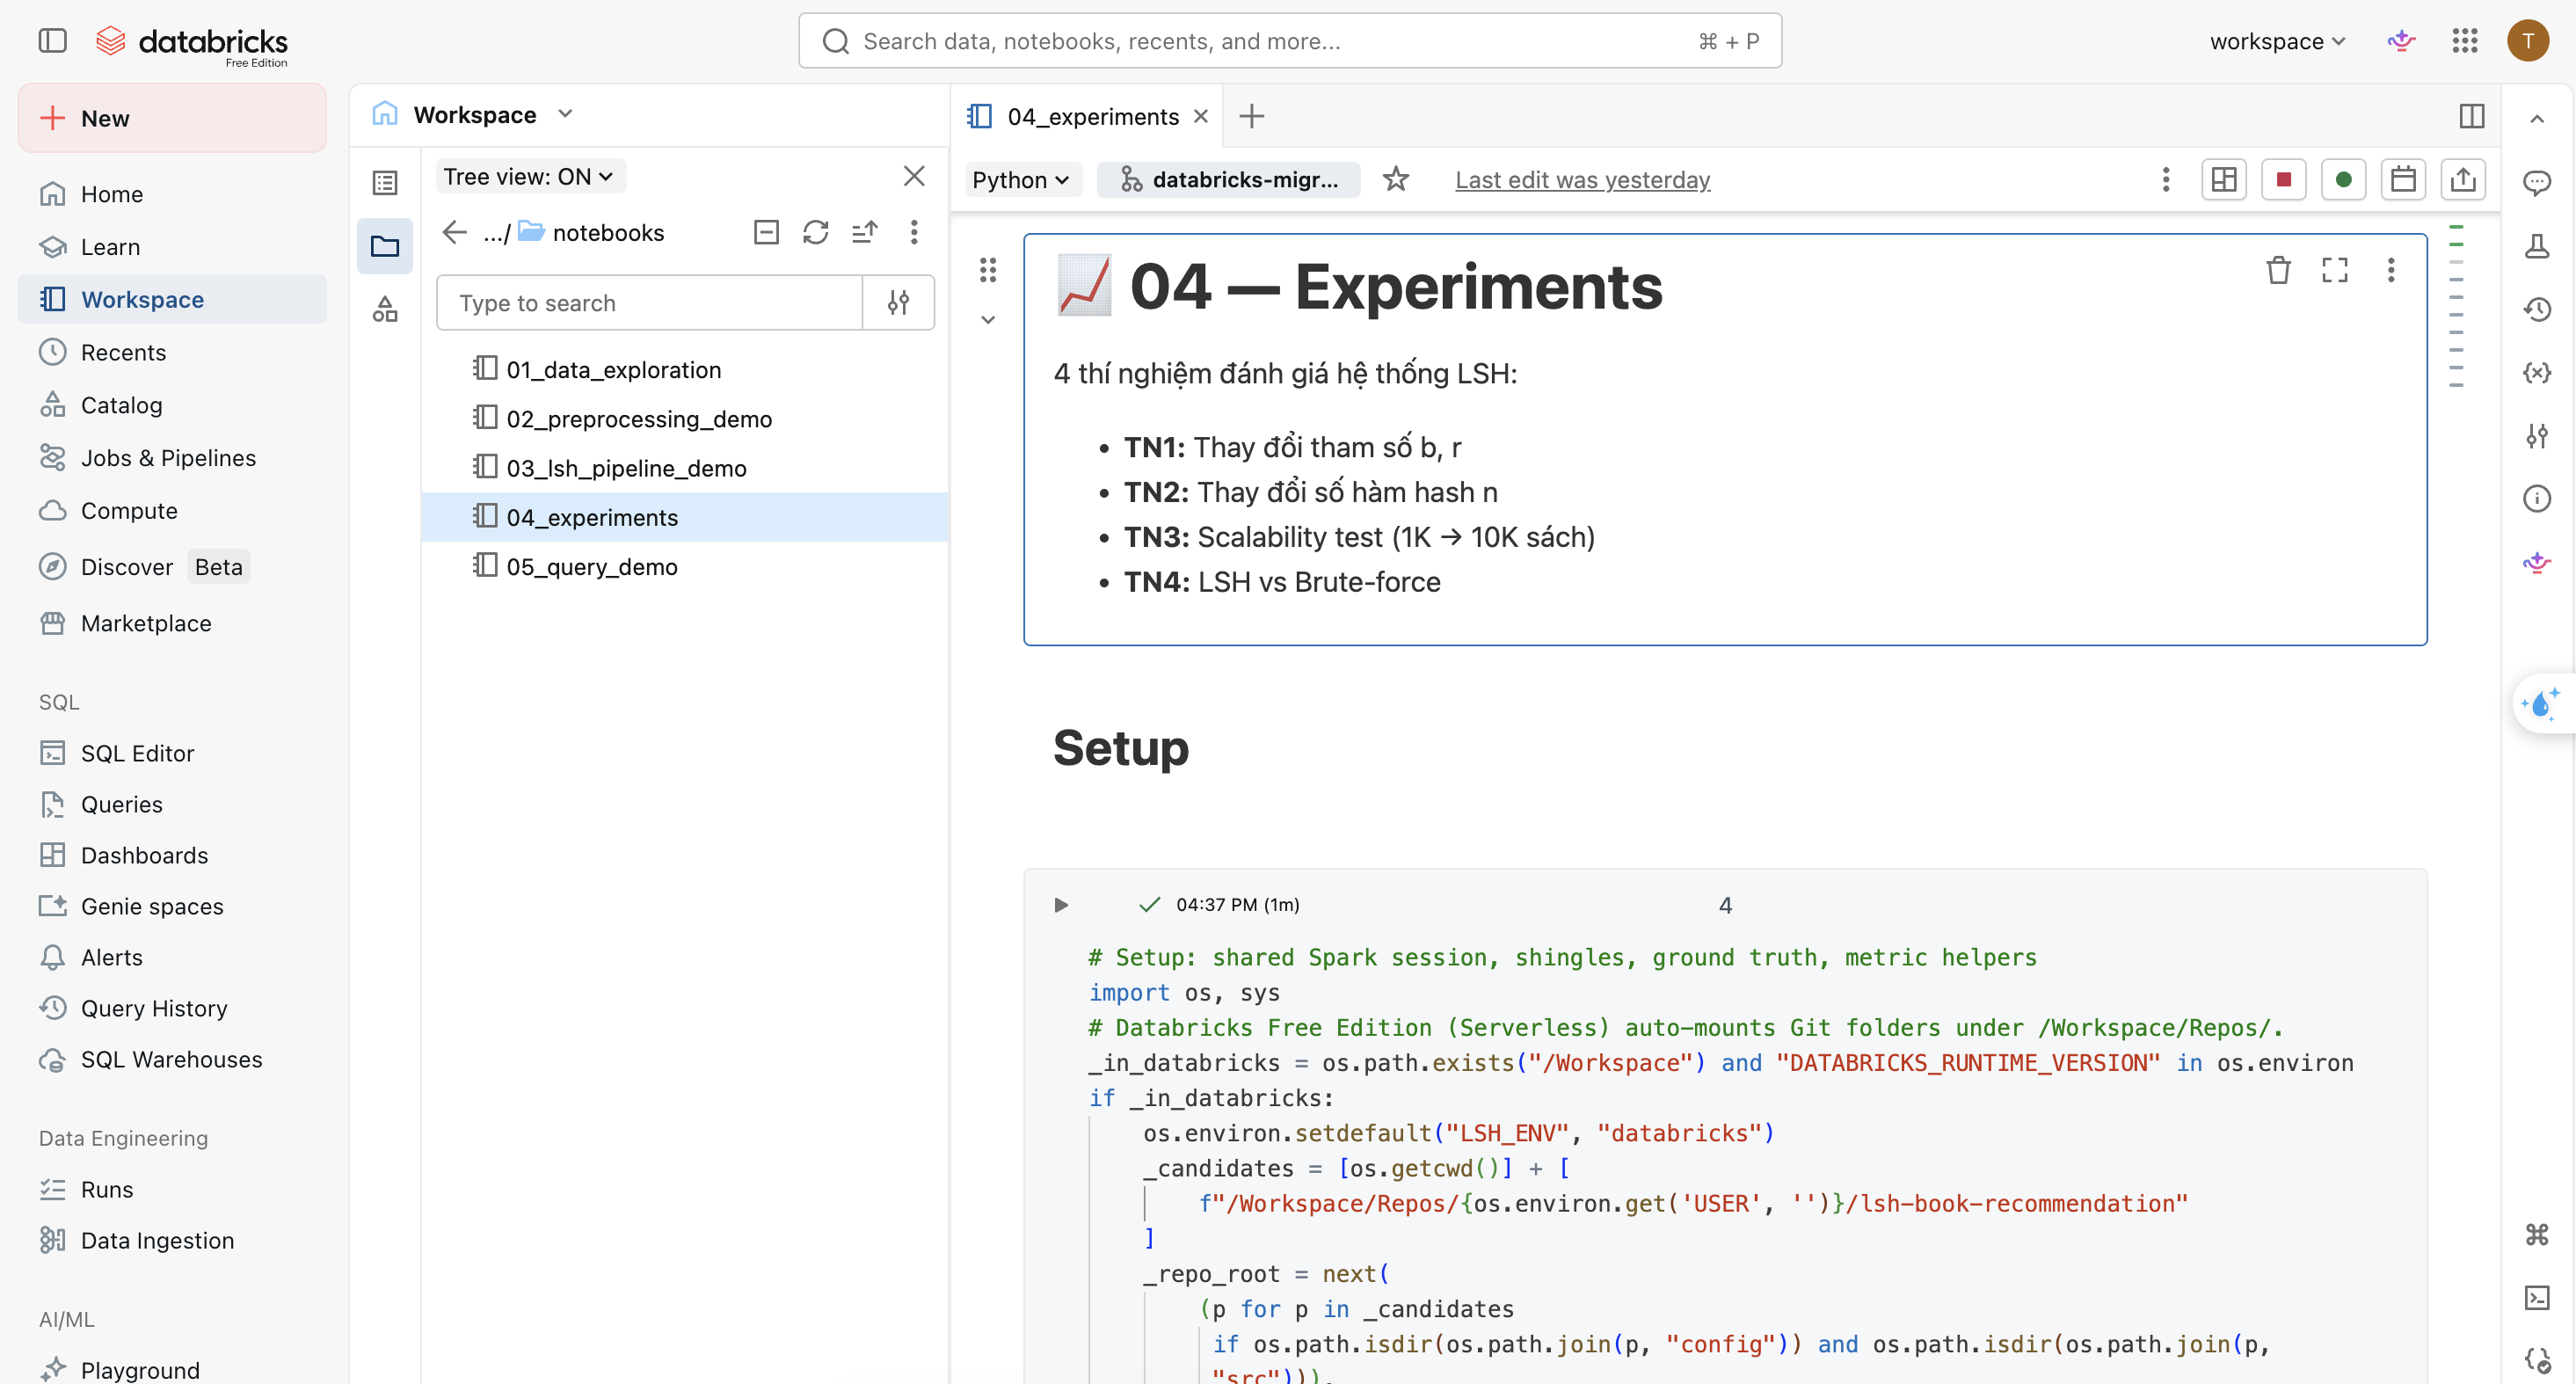
\includegraphics[width=0.7\linewidth]{Images/techstack/databricks.png}
    % \fbox{\parbox[c][3cm][c]{0.7\linewidth}{\centering\textit{[Placeholder: Logo Databricks hoặc screenshot Databricks workspace với notebook 04\_experiments --- sẽ chèn sau]}}}
    \caption{Databricks Free Edition (Serverless) --- runtime thực tế cho TN1--TN4}
    \label{fig:tech-databricks}
\end{figure}

\subsection{Apache Hadoop \& HDFS}

\textbf{Apache Hadoop} là framework mã nguồn mở cho lưu trữ và xử lý phân tán dữ liệu lớn, ra đời 2006 dựa trên paper Google File System (2003) và MapReduce (2004). \textbf{HDFS (Hadoop Distributed File System)} là tầng lưu trữ của Hadoop với các đặc tính:
\begin{itemize}
    \item \textbf{Block-based:} mỗi file chia thành block (mặc định 128 MB), nhân bản (replication factor mặc định $= 3$) trên nhiều DataNode để chịu lỗi.
    \item \textbf{Master-slave:} NameNode quản lý metadata + namespace, DataNode lưu trữ block thật. Cấu hình thiết kế: 1 NameNode + 2 DataNode.
    \item \textbf{Write-once read-many:} tối ưu cho batch analytics, không phù hợp với random update.
\end{itemize}

Trong project này, cấu trúc thư mục HDFS đã được thiết kế (xem Listing~\ref{lst:hdfs-structure} ở \S\ref{sec:implementation} cho layout đầy đủ \texttt{raw/cleaned/signatures/lsh\_index/metadata/results}); việc deploy thật bị blocked do thiếu cloud credits, được thay tạm bằng Databricks-managed storage và Volumes.

\begin{figure}[H]
    \centering
    % TODO: chèn ảnh — gợi ý: sơ đồ kiến trúc HDFS (NameNode + DataNodes) hoặc logo Hadoop
    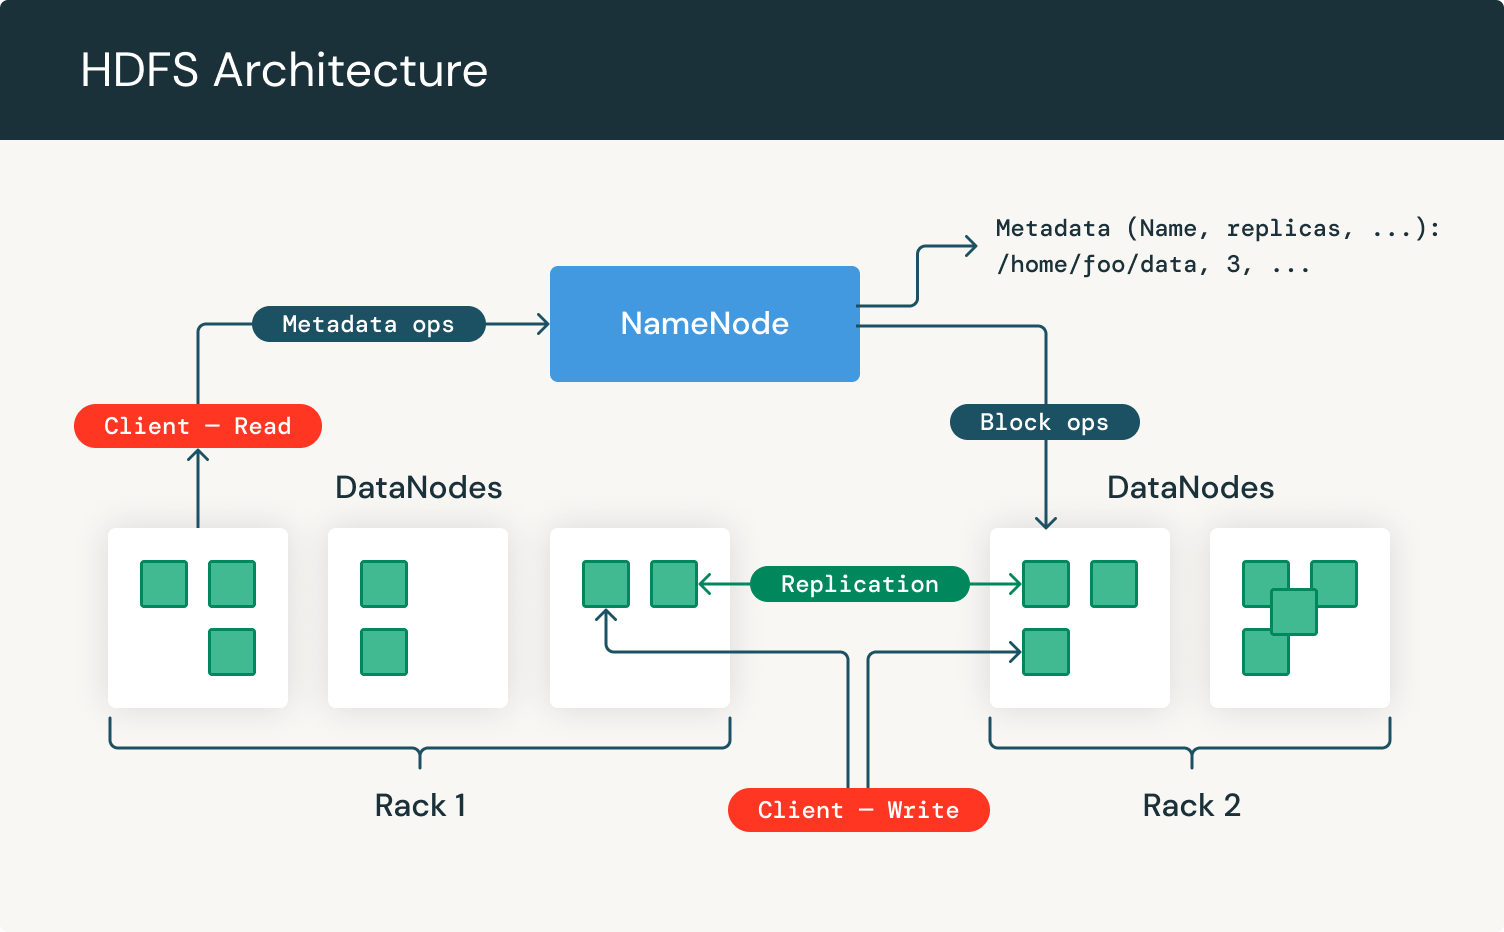
\includegraphics[width=0.7\linewidth]{Images/techstack/hadoop_hdfs.png}
    % \fbox{\parbox[c][3cm][c]{0.7\linewidth}{\centering\textit{[Placeholder: Sơ đồ kiến trúc HDFS (NameNode + DataNodes + block replication) hoặc logo Hadoop --- sẽ chèn sau]}}}
    \caption{Apache HDFS --- kiến trúc lưu trữ phân tán (thiết kế)}
    \label{fig:tech-hdfs}
\end{figure}

\subsection{Apache Parquet}

\textbf{Apache Parquet} là định dạng lưu trữ \textbf{columnar} mã nguồn mở, ra đời 2013 từ hợp tác giữa Twitter và Cloudera, trở thành Apache top-level project năm 2015. Khác với row-based format (CSV, JSON), Parquet lưu giá trị của cùng một cột liên tiếp nhau, mang lại 3 lợi thế cho workload analytic:
\begin{itemize}
    \item \textbf{Column pruning:} truy vấn chỉ cần một số cột $\rightarrow$ chỉ đọc đúng những column block cần thiết, giảm I/O.
    \item \textbf{Predicate pushdown:} filter theo giá trị cột được áp dụng ngay khi đọc file, nhờ min/max statistics lưu trong page footer.
    \item \textbf{Compression hiệu quả:} dữ liệu cùng kiểu trong một cột nén tốt hơn nhiều so với row-based; mặc định Snappy, hỗ trợ thêm gzip, zstd, lz4.
\end{itemize}

Trong project này, Parquet được dùng cho \texttt{tokens\_df}, \texttt{shingles\_df}, \texttt{minhash\_signatures}, và \texttt{lsh\_buckets}. Spark đọc/ghi Parquet native qua \texttt{spark.read.parquet(...)} / \texttt{df.write.parquet(...)}.

\begin{figure}[H]
    \centering
    % TODO: chèn ảnh — gợi ý: minh họa columnar vs row-based, hoặc logo Apache Parquet
    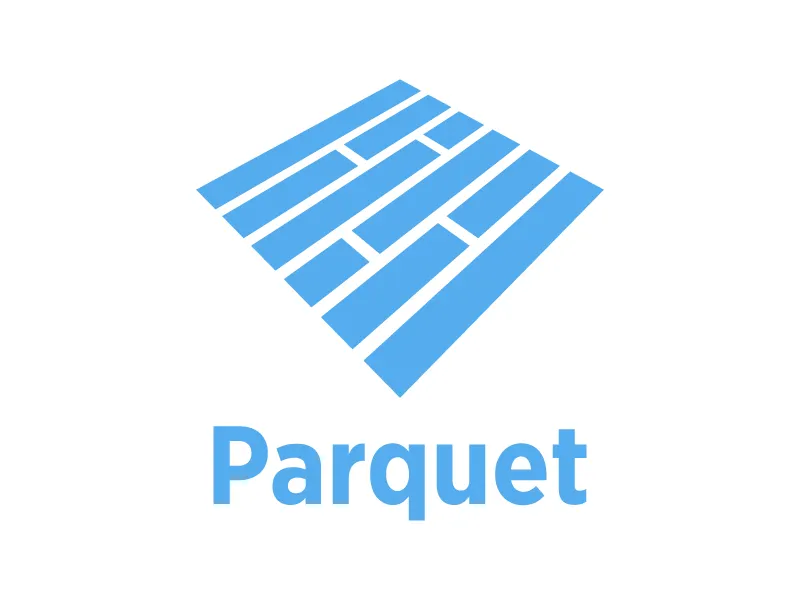
\includegraphics[width=0.7\linewidth]{Images/techstack/parquet.png}
    % \fbox{\parbox[c][3cm][c]{0.7\linewidth}{\centering\textit{[Placeholder: Minh họa columnar storage layout (cột vs hàng) hoặc logo Apache Parquet --- sẽ chèn sau]}}}
    \caption{Apache Parquet --- định dạng columnar cho intermediate data}
    \label{fig:tech-parquet}
\end{figure}

\subsection{Apache Spark \& PySpark}

\textbf{Apache Spark} là engine phân tích phân tán thống nhất, khởi nguồn từ UC Berkeley AMP Lab (2009) và trở thành Apache top-level project năm 2014. So với Hadoop MapReduce thế hệ trước, Spark đạt tốc độ nhanh hơn 10--100$\times$ nhờ \textbf{tính toán in-memory} và DAG scheduler tối ưu.

Các thành phần được sử dụng trong project:
\begin{itemize}
    \item \textbf{Spark SQL / DataFrame API:} biểu diễn shingles, signatures, LSH buckets dưới dạng DataFrame; transformations (map, flatMap, groupBy) chạy phân tán.
    \item \textbf{User-Defined Functions (UDFs):} hash family $h(x) = (ax + b) \bmod p$ trong MinHash được biểu diễn bằng PySpark UDFs.
    \item \textbf{PySpark:} binding Python qua Py4J bridge, cho phép code thuật toán bằng Python (\texttt{src/minhash.py}, \texttt{src/lsh.py}, \texttt{src/shingling.py}) trong khi engine vẫn chạy trên JVM.
\end{itemize}

Cluster manager: Spark hỗ trợ standalone / YARN / Mesos / Kubernetes; trong project, Databricks Serverless quản lý cluster lifecycle thay cho YARN ban đầu được dự kiến.

\begin{figure}[H]
    \centering
    % TODO: chèn ảnh — gợi ý: sơ đồ Driver/Executor/Cluster Manager hoặc logo Apache Spark
    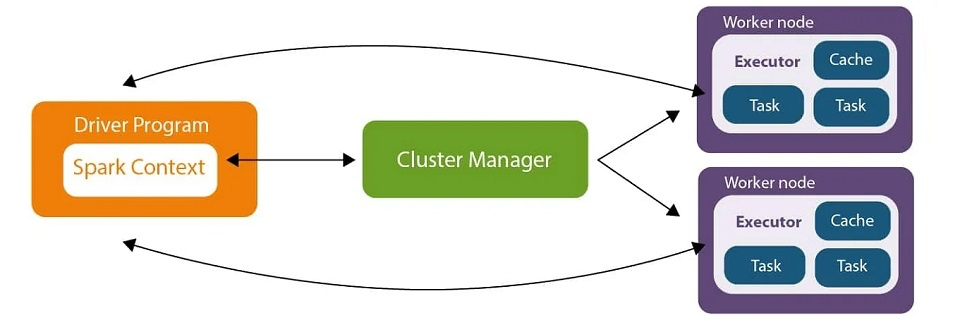
\includegraphics[width=0.7\linewidth]{Images/techstack/spark.png}
    % \fbox{\parbox[c][3cm][c]{0.7\linewidth}{\centering\textit{[Placeholder: Sơ đồ kiến trúc Apache Spark (Driver / Executor / Cluster Manager) hoặc logo Spark + PySpark --- sẽ chèn sau]}}}
    \caption{Apache Spark + PySpark --- engine xử lý phân tán}
    \label{fig:tech-spark}
\end{figure}

